%\section{Artificial Neural Networks}
%\subsection{NARX}
\label{sec:ANN:NARX}

Based on the linear ARX models, NARX ones have been demonstrated 
suitable for modeling nonlinear systems. Its defining general 
equation is
\begin{equation*}
\begin{split}
y(t) &=f(y(t-1),y(t-2),...,y(t-n_{a}), \\
&x(t-n_{k}),x(t-(n_{k}+1)),...,x(t-(n_{k}+n_{b})))
\end{split}
\end{equation*}
where the next value of the dependent output signal $y(t)$ is 
regressed on the $n_{a}$ previous values of the same output signal 
and $n_{b}$ previous values of the independent exogenous input 
signal $x(t)$. The prediction horizon $n_{k}$ is defined as the 
shift among corresponding input and output values so that current 
input is used for predicting the output in $n_{k}$ time steps in the 
future. The unique dissimilarity with the ARX models lies in the 
non-linearity of the function $f$. 

We implemented the NARX neural network with the Neural Network 
Toolbox of MatLab. In order to adapt the topology to our scenario, 
we configured the network with four exogenous inputs (HR, EDA, 
temperature and SpO2). We used as output signal of the system a line 
whose slope is determined by the time interval between the 
beginnings of the aura and pain phases. With this line we try to 
predict the upward slope of the symptomatic curve of probability we 
have just modelled. 

\begin{figure}[!ht]
\centering
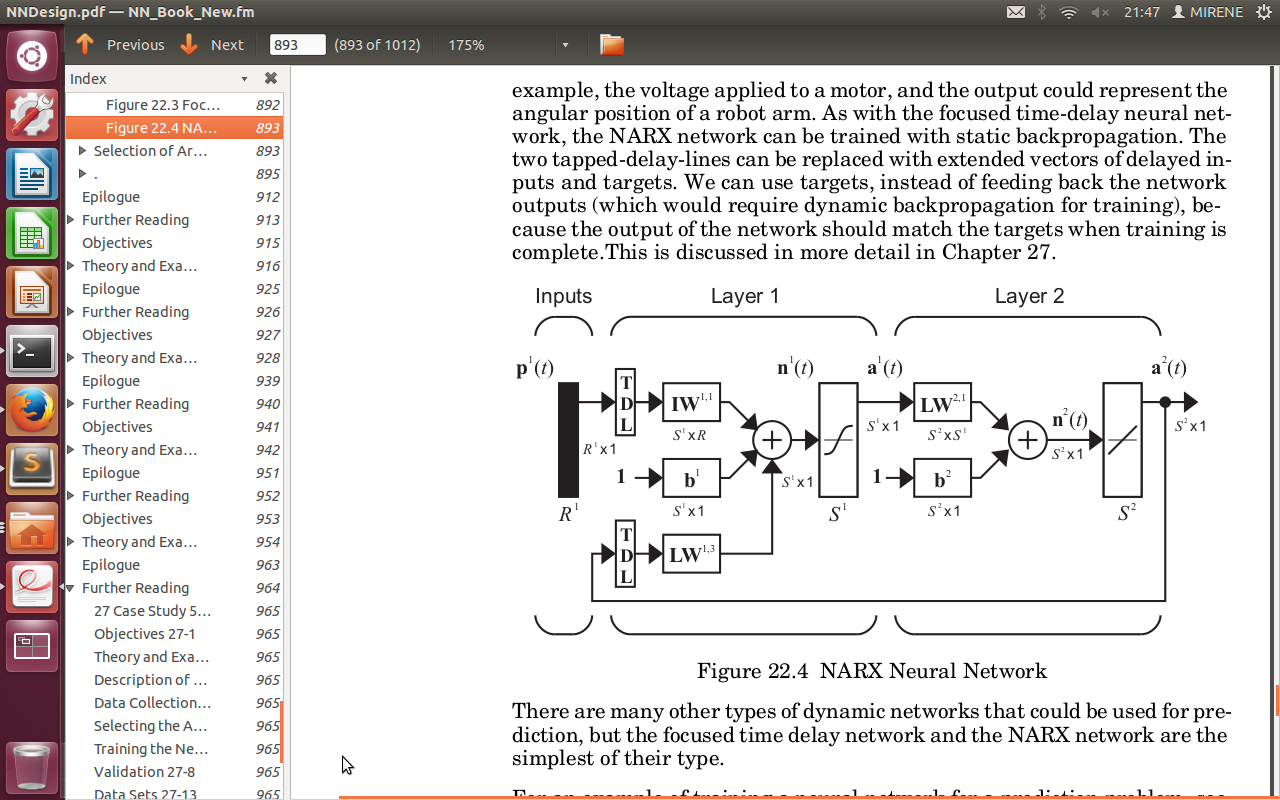
\includegraphics[width=0.5\textwidth]{images/narx.png}
\caption{NARX network}
\label{fig:narx}
\end{figure}


The used NARX network counts with one hidden layer with 10 
neurons apart from the input and output layers. 
The memory feature is included with a tapped delay line at input. 
The activation function of the hidden layer was established as 
a \textit{tansig}, whereas the one used in the output layer is 
a \textit{purelin}. Then, in order to obtained values in the range of [0,1], values lower than 0 were fixed to 0 and the ones greater than 1 to a value of 1.

Another consideration to take into account is that we trained the 
NARX network in open loop, in which the true output is used instead 
of feeding back the estimated output. The NARX network was then 
converted to the closed loop configuration for validating and 
testing the model.

The training set consists on one, two or three migraines and then we tested the model with the four migraines we had at our disposal. 
We iteratively checked the perform  
of the possible combinations of values of 
$n_{a}$, $n_{b}$ and $n_{k}$, where $n_{a} = n_{b}$ to reduce
complexity. As the weights of the neurons were randomly initialized,
we created several nets with the same configuration and initialized
and trained each one independently. Then, we compared the results
and stored the best one.

%%%%%%%%%%%%%%%%%%%%%%%%%%%%%%%%%%%%%%%%%%%
%%%%%%%%%%%%% ESTO DEBERÍA IR DONDE LOS RESULTADOS
After checking iteratively the perform  
of the possible combinations of values of 
$n_{a}=n_{b}$ and $n_{k}$, with different training and testing
sets, the best NARX model with ANN was obtained when the net was 
trained with three migraines, with $n_{k}=10$ and $n_{a}=6=n{b}$.
In order to avoid false positives, we fixed a threshold 
of probability of detection of 0.5. The margin of prediction is then 
defined as the sum of the $n_{k}$ value and the time interval 
between the instant when the prectictive curve reaches the threshold 
and the begining of the aura. The resultant graphic 
(\figref{narxTest})
shows that we gain a range of 100-200 extra
minutes for predicting. In contrast, the system must be restarted
every time a migraine is detected since it maintains its high level 
response indefinitely. This would be one of the aspects to improve 
in further works.

\begin{figure}
\centering
\includegraphics[width=\columnwidth]{narxTest_graph}
\caption{NARX model test for a migraine not used in training}
\label{fig:narxTest}
\end{figure}

